\documentclass{article}

% Language setting
% Replace `english' with e.g. `spanish' to change the document language
\usepackage[english]{babel}

% Set page size and margins
% Replace `letterpaper' with `a4paper' for UK/EU standard size
\usepackage[letterpaper,top=2cm,bottom=2cm,left=3cm,right=3cm,marginparwidth=1.75cm]{geometry}

% Useful packages
\usepackage{amsmath}
\usepackage{graphicx}
\usepackage[colorlinks=true, allcolors=blue]{hyperref}
\usepackage{amstext} % for \text macro
\usepackage{array}   % for \newcolumntype macro
\newcolumntype{L}{>{$}l<{$}} % math-mode version of "l" column type
\usepackage{makecell}
\usepackage{caption}

\usepackage[version=4]{mhchem}
\usepackage{stmaryrd}
\usepackage[export]{adjustbox}
\usepackage{tikz}

\usepackage[outline]{contour}
\contourlength{0.25pt}

\usepackage{listings} %For code in appendix
\lstset
{ %Formatting for code in appendix
    language=C++,
    basicstyle=\footnotesize,
    numbers=left,
    stepnumber=1,
    showstringspaces=false,
    tabsize=2,
    breaklines=true,
    breakatwhitespace=false,
}

\usepackage{mathtools}
\DeclarePairedDelimiter\ceil{\lceil}{\rceil}
\DeclarePairedDelimiter\floor{\lfloor}{\rfloor}
\newcommand{\red}[1]{\textcolor{red}{#1}}

\title{DSA. Problem solutions. Week 8.}
\author{You}

\begin{document}
\maketitle


% TASK 1
\section{Task 1}
\subsection{Statement}
Insert the ⟨key, value⟩ items into an empty B-tree [Cormen, §18] with minimum degree $t = 2$:
\begin{enumerate}
    \item [(a)] ⟨33, U⟩, ⟨10, T⟩, ⟨17, I⟩, ⟨12, N⟩, ⟨23, U⟩
    \item [(b)] ⟨1, A⟩, ⟨29, D⟩, ⟨36, Y ⟩, ⟨3, S⟩, ⟨5, T⟩
    \item [(c)] ⟨19, P⟩, ⟨14, O⟩, ⟨7, I⟩, ⟨8, N⟩, ⟨39, I⟩
    \item [(d)]  ⟨27, I⟩, ⟨35, N⟩, ⟨20, O⟩, ⟨25, L⟩, ⟨31, S⟩
\end{enumerate}

Show the state of the tree after every 5 insertions. Depict each tree as a sequence of arrays for
each layer. For example, consider this B-tree:

\begin{center}
  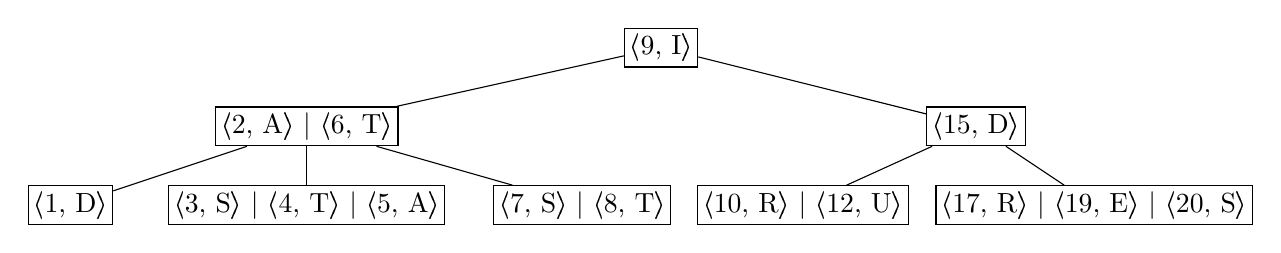
\begin{tikzpicture}
  \node[rectangle, draw = black, inner sep=2px] (A) at (0,0) {⟨9, I⟩};
  \node[rectangle, draw, inner sep=2px] (B) at (-4.5,-1) {⟨2, A⟩ $\vert$ ⟨6, T⟩};
  \node[rectangle, draw, inner sep=2px] (C) at (4,-1) {⟨15, D⟩};
  \node[rectangle, draw, inner sep=2px] (D) at (-7.5,-2) {⟨1, D⟩};
  \node[rectangle, draw, inner sep=2px] (E) at (-4.5,-2) {⟨3, S⟩ $\vert$ ⟨4, T⟩ $\vert$ ⟨5, A⟩};
  \node[rectangle, draw, inner sep=2px] (F) at (-1, -2) {⟨7, S⟩ $\vert$ ⟨8, T⟩};
  \node[rectangle, draw, inner sep=2px] (G) at (1.8, -2) {⟨10, R⟩ $\vert$ ⟨12, U⟩};
  \node[rectangle, draw, inner sep=2px] (H) at (5.5, -2) {⟨17, R⟩ $\vert$ ⟨19, E⟩ $\vert$ ⟨20, S⟩};
  \draw (A) -- (B);
  \draw (A) -- (C);
  \draw (B) -- (D);
  \draw (B) -- (E);
  \draw (B) -- (F);
  \draw (C) -- (G);
  \draw (C) -- (H);
  \end{tikzpicture}
\end{center}

The tree above must be depicted as follows:
\setlength{\tabcolsep}{3pt}
\begin{enumerate}

    \item [(layer 1)]
        \begin{tabular}{|c|}
            \hline
             ⟨9, I⟩ \\
             \hline
        \end{tabular} \;
        
    \item [(layer 2)]
        \begin{tabular}{|c|c|}
            \hline
             ⟨2, A⟩ & ⟨6, T⟩ \\
            \hline
        \end{tabular} \;
        \begin{tabular}{|c|}
            \hline
             ⟨15, D⟩ \\
            \hline
        \end{tabular} \;
        
    \item [(layer 3)]
        \begin{tabular}{|c|}
            \hline
             ⟨1, D⟩ \\
            \hline
        \end{tabular} \;
        \begin{tabular}{|c|c|c|}
            \hline
             ⟨3, S⟩ & ⟨4, T⟩ & ⟨5, A⟩ \\
            \hline
        \end{tabular} \;
        \begin{tabular}{|c|c|}
            \hline
             ⟨7, S⟩ & ⟨8, T⟩ \\
            \hline
        \end{tabular} \;
        \begin{tabular}{|c|c|}
            \hline
             ⟨10, R⟩ & ⟨12, U⟩ \\
            \hline
        \end{tabular} \;
        \begin{tabular}{|c|c|c|}
            \hline
             ⟨17, R⟩ & ⟨19, E⟩ & ⟨20, S⟩ \\
            \hline
        \end{tabular} \;
\end{enumerate}

\subsection{Answer}
\begin{enumerate}
    \item Insertion 1
    \begin{enumerate}
        \item [(layer 1)]
            \begin{tabular}{|c|}
                \hline
                 ⟨9, I⟩ \\
                 \hline
            \end{tabular} \;
        \item [(layer 2)]
            \begin{tabular}{|c|c|}
                \hline
                 ⟨2, A⟩ & ⟨6, T⟩ \\
                \hline
            \end{tabular} \;
            \begin{tabular}{|c|}
                \hline
                 ⟨15, D⟩ \\
                \hline
            \end{tabular} \;
    \end{enumerate}
    
    \item Insertion 2
    \begin{enumerate}
        \item [(layer 1)]
            \begin{tabular}{|c|}
                \hline
                 ⟨9, I⟩ \\
                 \hline
            \end{tabular} \;
        \item [(layer 2)]
            \begin{tabular}{|c|c|}
                \hline
                 ⟨2, A⟩ & ⟨6, T⟩ \\
                \hline
            \end{tabular} \;
            \begin{tabular}{|c|}
                \hline
                 ⟨15, D⟩ \\
                \hline
            \end{tabular} \;
    \end{enumerate}
    
    \item Insertion 3
    \begin{enumerate}
        \item [(layer 1)]
            \begin{tabular}{|c|}
                \hline
                 ⟨9, I⟩ \\
                 \hline
            \end{tabular} \;
        \item [(layer 2)]
            \begin{tabular}{|c|c|}
                \hline
                 ⟨2, A⟩ & ⟨6, T⟩ \\
                \hline
            \end{tabular} \;
            \begin{tabular}{|c|}
                \hline
                 ⟨15, D⟩ \\
                \hline
            \end{tabular} \;
    \end{enumerate}
    
    \item Insertion 4
    \begin{enumerate}
        \item [(layer 1)]
            \begin{tabular}{|c|}
                \hline
                 ⟨9, I⟩ \\
                 \hline
            \end{tabular} \;
        \item [(layer 2)]
            \begin{tabular}{|c|c|}
                \hline
                 ⟨2, A⟩ & ⟨6, T⟩ \\
                \hline
            \end{tabular} \;
            \begin{tabular}{|c|}
                \hline
                 ⟨15, D⟩ \\
                \hline
            \end{tabular} \;
    \end{enumerate}
\end{enumerate}
\setlength{\tabcolsep}{6pt}


% TASK 2
\section{Task 2}
\subsection{Statement}
Perform Heap-Sort [Cormen, §6.4] on the following input array:

\begin{table}[!h]
    \centering
    \begin{tabular}{|c|c|c|c|c|c|c|c|c|}
        \hline
        1 & 3 & 7 & 8 & 0 & 2 & 5 & 4 & 6 \\
        \hline
    \end{tabular}
\end{table}

Show the state of the array after each call to Max-Heapify (solution must have 12 arrays).

\subsection{Answer}

\begin{table}[!h]
    \centering
    \begin{tabular}{|c||c|c|c|c|c|c|c|c|c|}
        \hline
        Call 1 & 1 & 3 & 7 & 8 & 0 & 2 & 5 & 4 & 6 \\
        \hline
        Call 2 & 1 & 3 & 7 & 8 & 0 & 2 & 5 & 4 & 6 \\
        \hline
    \end{tabular}
\end{table}


% TASK 3
\section{Task 3}
\subsection{Statement}
(+1\% extra credit) A $d$-ary heap is similar to a binary heap, except non-leaf nodes have $d$ children instead of 2 children (except the last non-leaf node, which is allowed to have fewer children). Adjust the array representation and the efficient implementations of Max-Heapify and Build-Max-Heap. Perform Heap-Sort [Cormen, §6.4] but using a 3-ary heap on the following input array:

\begin{table}[!h]
    \centering
    \begin{tabular}{|c|c|c|c|c|c|c|c|c|}
        \hline
        1 & 3 & 7 & 8 & 0 & 2 & 5 & 4 & 6 \\
        \hline
    \end{tabular}
\end{table}

Show the state of the array after each call to Max-Heapify (solution must have 11 arrays).


\subsection{Answer}

\begin{table}[!h]
    \centering
    \begin{tabular}{|c||c|c|c|c|c|c|c|c|c|}
        \hline
        Call 1 & 1 & 3 & 7 & 8 & 0 & 2 & 5 & 4 & 6 \\
        \hline
        Call 2 & 1 & 3 & 7 & 8 & 0 & 2 & 5 & 4 & 6 \\
        \hline
    \end{tabular}
\end{table}


\section*{References}
[Cormen] T. H. Cormen, C. E. Leiserson, R. L. Rivest and C. Stein. Introduction to Algorithms, Fourth Edition. The MIT Press 2022

[Goodrich] M. T. Goodrich, R. Tamassia, and M. H. Goldwasser. Data Structures and Algorithms in Java. WILEY 2014.

\end{document}
